\section{Secondo Esercizio}\label{Sec:SecondoEsercizio}
Sensore Resistometrico
\begin{figure}[h]
    \centering
    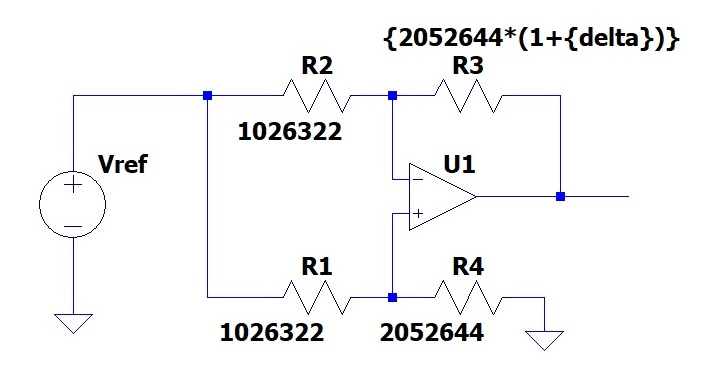
\includegraphics[width=0.9\textwidth]{Figure/Circuito2.jpg}
    \caption{Circuito del secondo esercizio}
    \label{fig:Circuito2}
\end{figure}\\
Listato SPICE della rete considerata:\\
\\
XU1 N002 N004 N003 opamp Aol=100K GBW=10Meg\\
R1 N004 N001 1026322\\
R2 N002 N001 1026322\\
R3 N003 N002 {2052644*(1+{delta})}\\
R4 0 N004 2052644\\
Vref N001 0\\
.inc opamp.sub\\
.step param delta 0 1 0.1\\
.dc Vref 0 -18.75 0.5\\
.backanno\\
.end\\

\subsection{Analisi Analitica}\label{subsec:analisiAnaliticaSecondo}
Per una Vref generica cerchiamo la relazione tra ingresso e uscita del circuito
\begin{itemize}
\item 
    \begin{equation}\label{eq:eqMorsettiAmplificatoreSecondo}
    V_{-} = V_{+} = V_{ref} \dfrac{R}{R_{1} + R}
    \end{equation}
\item 
    \begin{equation}\label{eq:eqCorrenteRSecondo}
    I_{R_{1+\delta}} = \dfrac{V_{-} - V_{ref}}{R_{1}} = \dfrac{V_{ref}}{R_{1}} ( \dfrac{R}{R_{1} + R} - 1 )
    \end{equation}
\item
    \begin{equation}\label{eq:eqTensioneUscitaSecondo1}
    V_{out} = I_{R(1+\delta)} R(1+\delta) + V_{-}
    \end{equation}
    \begin{equation}\label{eq:eqTensioneUscitaSecondo2}
    V_{out} = V_{ref} \dfrac{R(1+\delta)}{R_{1}}(\dfrac{R}{R_{1} + R} - 1) + V_{ref} \dfrac{R}{R_{1} + R}
    \end{equation}
    \begin{equation}\label{eq:eqTensioneUscitaSecondo3}
    V_{out} = V_{ref} (\dfrac{-R_{1}}{R_{1} + R} \dfrac{R(1+\delta)}{R_{1}} + \dfrac{R}{R_{1} + R})  
    \end{equation}
    \begin{equation}\label{eq:eqTensioneUscitaSecondo4}
    V_{out} = V_{ref} (-\dfrac{R}{R_{1} + R} -\dfrac{R\delta}{R_{1} + R} + \dfrac{R}{R_{1} + R}) = - V_{ref} \dfrac{R}{R_{1} + R} \delta 
    \end{equation}
\end{itemize}

\subsection{Dimensionamento del Circuito}\label{subsec:dimensionamentoCircuito}
Come trovato nella formula \ref{eq:eqTensioneUscitaSecondo4} la relazione tra tensione di uscita e tensione di ingresso è la seguente $$V_{out} = - V_{ref} \dfrac{R}{R_{1} + R} \delta$$
Andiamo ora a dimensionare il circuito in modo che $$V_{out} = 12,5 \delta$$
Fissiamo le resistenze
$$R = 2052644$$
$$R_{1} = \dfrac{R}{2} = 1026322$$
Ricaviamo quindi la tensione del generatore in ingresso
\begin{equation}\label{eq:eqTensioneIngresso}
V_{ref} = -12,5\dfrac{R_{1} + R}{R} = -12,5\dfrac{3}{2} = -18,75 V
\end{equation}

\subsection{Corrente attraverso Sensore Resistometrico}\label{subsec:correnteSensoreResistometrico}
Simulando con SPICE il circuito e facendo variare la tensione in ingresso e il parametro variabile del sensore resistometrico otteniamo il seguente grafico per la corrente che scorre nella resistenza.
\begin{figure}[h]
    \centering
    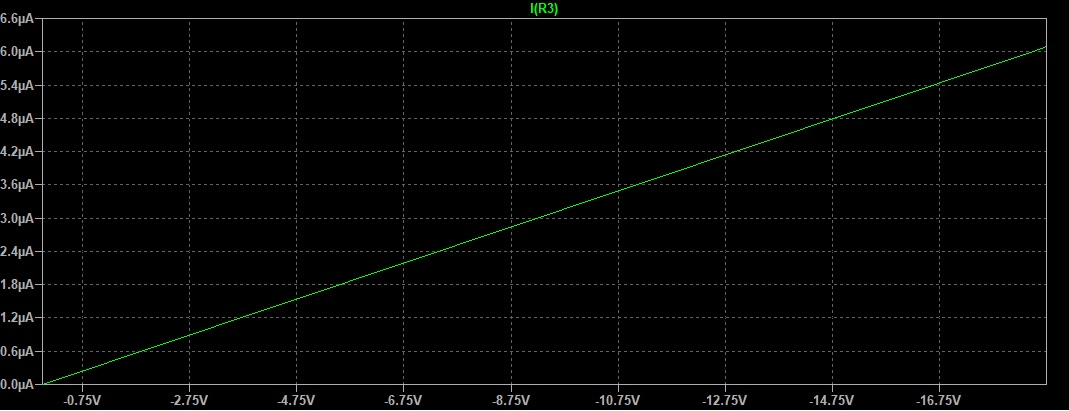
\includegraphics[width=1\textwidth]{Figure/UscitaCorrente.jpg}
    \caption{Corrente che attraversa il sensore resistometrico}
    \label{fig:correnteSensoreResistometrico}
\end{figure}
